\documentclass[tikz,border=4pt]{standalone}
\usetikzlibrary{positioning, shapes.geometric, arrows.meta}

\tikzset{
  base/.style     = {draw, thick, minimum width=28mm, minimum height=9mm, align=center},
  terminal/.style = {base, rounded corners=4.5mm, fill=teal!15},
  process/.style  = {base, fill=blue!8},
  decision/.style = {base, diamond, aspect=2.2, inner sep=1pt, fill=orange!15},
  >={Stealth[length=2.5mm]},
}

\begin{document}
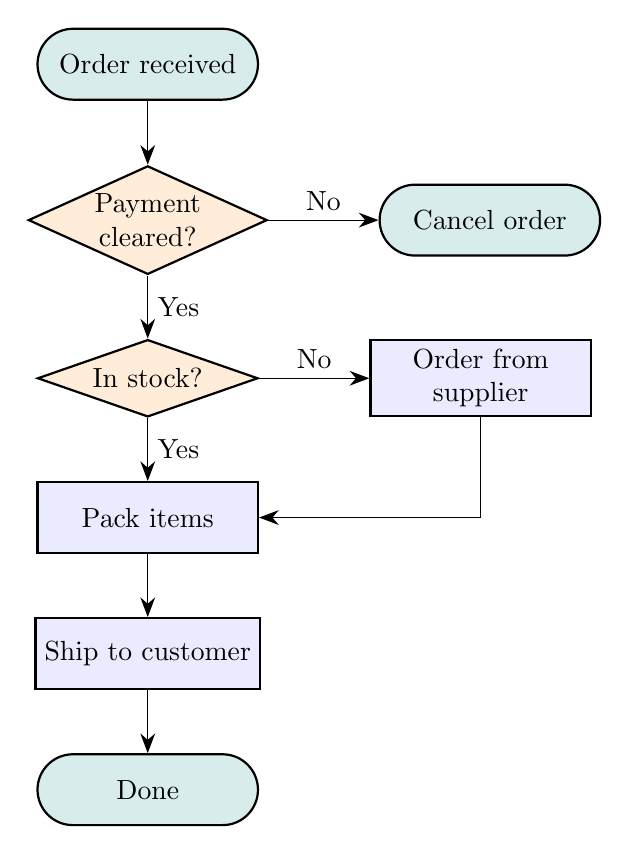
\begin{tikzpicture}[node distance=8mm and 14mm]
  \node[terminal]                  (start)  {Order received};
  \node[decision]  (paid) at (0,-1.98)   {Payment\\ cleared?};
  \node[terminal, right=of paid]   (cancel) {Cancel order};
  \node[decision, below=of paid]   (stock)  {In stock?};
  \node[process, right=of stock]   (supply) {Order from\\ supplier};
  \node[process, below=of stock]   (pack)   {Pack items};
  \node[process, below=of pack]    (ship)   {Ship to customer};
  \node[terminal, below=of ship]   (done)   {Done};

  \draw[->] (start)  -- (paid);
  \draw[->] (paid)   -- node[above] {No}  (cancel);
  \draw[->] (paid)   -- node[right] {Yes} (stock);
  \draw[->] (stock)  -- node[above] {No}  (supply);
  \draw[->] (stock)  -- node[right] {Yes} (pack);
  % The two branches meet again at "Pack items".
  \draw[->] (supply) |- (pack);
  \draw[->] (pack)   -- (ship);
  \draw[->] (ship)   -- (done);
\end{tikzpicture}
\end{document}
